%%%%%%%%%%%%%%%%%%%%%%%%%%%%%%%%%%%%%%%%%%%%%%%%%%%%%%%%%%%%%%%%%%%%%%%%%%%

\documentclass{standalone}

\usepackage{amsmath}
\usepackage{mathptmx}
\usepackage{pgfplots}
\usetikzlibrary{external}
\tikzexternalize{cricket-duck-linear}
\pgfplotsset{compat=1.16}

%% IEEE uses Times Roman font, so we'll default to Times.
%% These three commands make up the entire times.sty package.
\renewcommand{\rmdefault}{ptm}
\renewcommand{\ttdefault}{pcr}
\normalfont\selectfont

\begin{document}

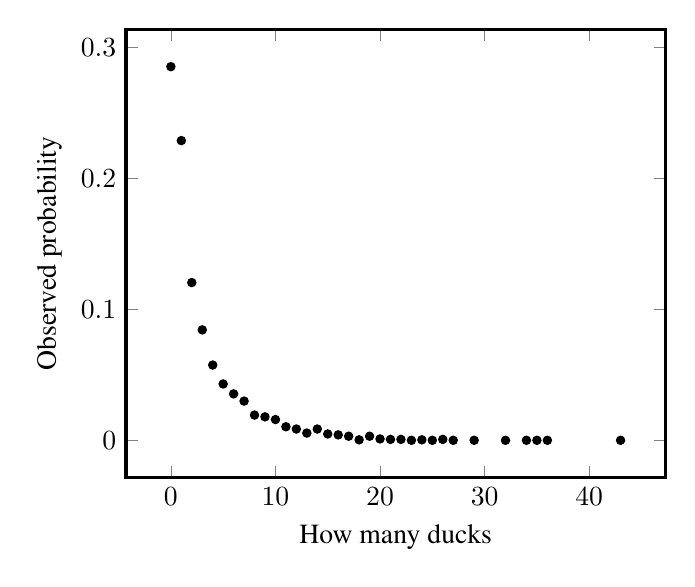
\begin{tikzpicture}
\tikzset{%%
  every mark/.append style={scale=1.0},%%
  scale=1.0%%
}
\pgfplotsset{%%
  every axis/.append style={font=\normalsize}%%
}
%%
\begin{axis}[%%
  axis line style=very thick,%%
  dotStyle/.style={mark size=1.5,black,mark color=black,mark=*,only marks},%%
  enlargelimits=true,%%
  %% x axis
  xlabel={\normalsize How many ducks},%%
  %% y axis
  ylabel={\normalsize Observed probability}%%
]
%%
%%
\addplot[dotStyle] coordinates {
  (0, 0.285223367697594)
  (1, 0.228865979381443)
  (2, 0.120618556701031)
  (3, 0.084536082474227)
  (4, 0.057731958762887)
  (5, 0.043298969072165)
  (6, 0.03573883161512)
  (7, 0.030240549828179)
  (8, 0.019587628865979)
  (9, 0.018213058419244)
  (10, 0.016151202749141)
  (11, 0.010652920962199)
  (12, 0.00893470790378)
  (13, 0.005841924398625)
  (14, 0.00893470790378)
  (15, 0.005154639175258)
  (16, 0.00446735395189)
  (17, 0.003436426116838)
  (18, 0.000687285223368)
  (19, 0.003436426116838)
  (20, 0.001374570446735)
  (21, 0.001030927835052)
  (22, 0.001030927835052)
  (23, 0.000343642611684)
  (24, 0.000687285223368)
  (25, 0.000343642611684)
  (26, 0.001030927835052)
  (27, 0.000343642611684)
  (29, 0.000343642611684)
  (32, 0.000343642611684)
  (34, 0.000343642611684)
  (35, 0.000343642611684)
  (36, 0.000343642611684)
  (43, 0.000343642611684)
};
\end{axis}
\end{tikzpicture}

\end{document}
